\documentclass{article}

\usepackage{tikz}
\usetikzlibrary{automata, positioning}
\begin{document}
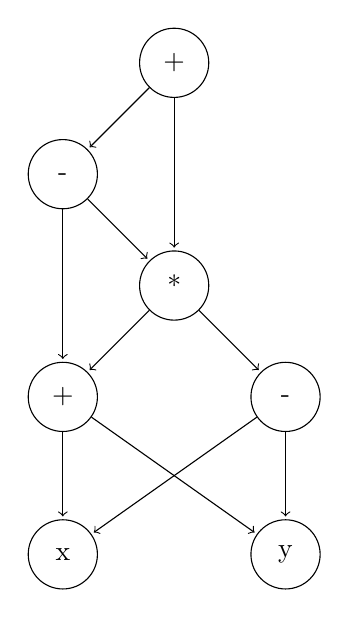
\begin{tikzpicture}[shorten >= 1pt, node distance = 2cm, on grid, auto]
  \node[state] (0) {+};
  \node[state] (1) [below left=of 0] {-};
  \node[state] (2) [below right=of 1] {*};
  \node[state] (3) [below left=of 2] {+};
  \node[state] (4) [below right=of 2] {-};
  \node[state] (5) [below=of 3] {x};
  \node[state] (6) [below=of 4] {y};
  \path[->]
    (0) edge node {} (1)
        edge node {} (2)
    (1) edge node {} (2)
        edge node {} (3)
    (2) edge node {} (3)
        edge node {} (4)
    (3) edge node {} (5)
        edge node {} (6)
    (4) edge node {} (5)
        edge node {} (6);
\end{tikzpicture}
\end{document}
